\chapter{Architecture and Design}
\label{chapter:architecture}

Before we reach the point of proposing a new future-proof, modern architecture, we first focus on the evolution of the Tribler architecture throughout the last decade of research. Better understanding of the architectural and design decisions that have been taken in the past, will help us to shed light on the question what contributed to the current state of the Tribler system.\\\\
According to the OpenHub tool\cite{openhubtribler} which accumulates statistics about many open source projects available on the Internet, Tribler received code contributions from 111 unique contributors so far. This list is most likely not exhaustive since some work of contributors might have been finished by other members of the Tribler team or has never been merged into the main code base. A query for \emph{Tribler} in the repository of Delft University of Technology\footnote{http://repository.tudelft.nl}, yields a total of 66 search results, consisting of 35 results which are contributions in the form of a MSc or BSc thesis and 31 research-oriented papers in the form of a PhD dissertation or (published) research work.\\\\
The remainder of this Chapter will present a historical view of the evolution of the Tribler platform, starting in 2007 and concluding with the proposal of a new, robust and scalable architecture that is ready for the next decade of research.

\section{Tribler in 2007: A social-based peer-to-peer system}
In April 2005, Tribler started out as a fork of the \emph{Another BitTorrent Client (ABC)} application, an improved BitTorrent client. ABC is based on \emph{BitTornado} which extended from the \emph{BitTorrent} core system, originally written by Bram Cohen. ABC was shipped with an user interface and a variety of features to manage BitTorrent downloads. The software makes use of the BitTorrent engine, at that time completely written in Python like the rest of ABC. This is most probably the reason why Python is used for Tribler development.\\\\
In 2007, the first major research paper was published, describing Tribler as a social-based peer-to-peer system\cite{pouwelse2008tribler}. The key idea as described in the paper is that social connections between peers in a decentralized network can be exploited to increase usability and performance of the network. This is based on the idea that peers belonging to a social group are not likely to steal (free-ride) bandwidth from each other. Free-riding is a phenomena that is widely observed in the regular BitTorrent network. The system architecture of Tribler as described in the work of Pouwelse et al. is presented in Figure \ref{fig:tribler-architecture-2008}. We will now highlight the most important parts of the given architecture.

\begin{figure}[t]
	\centering
	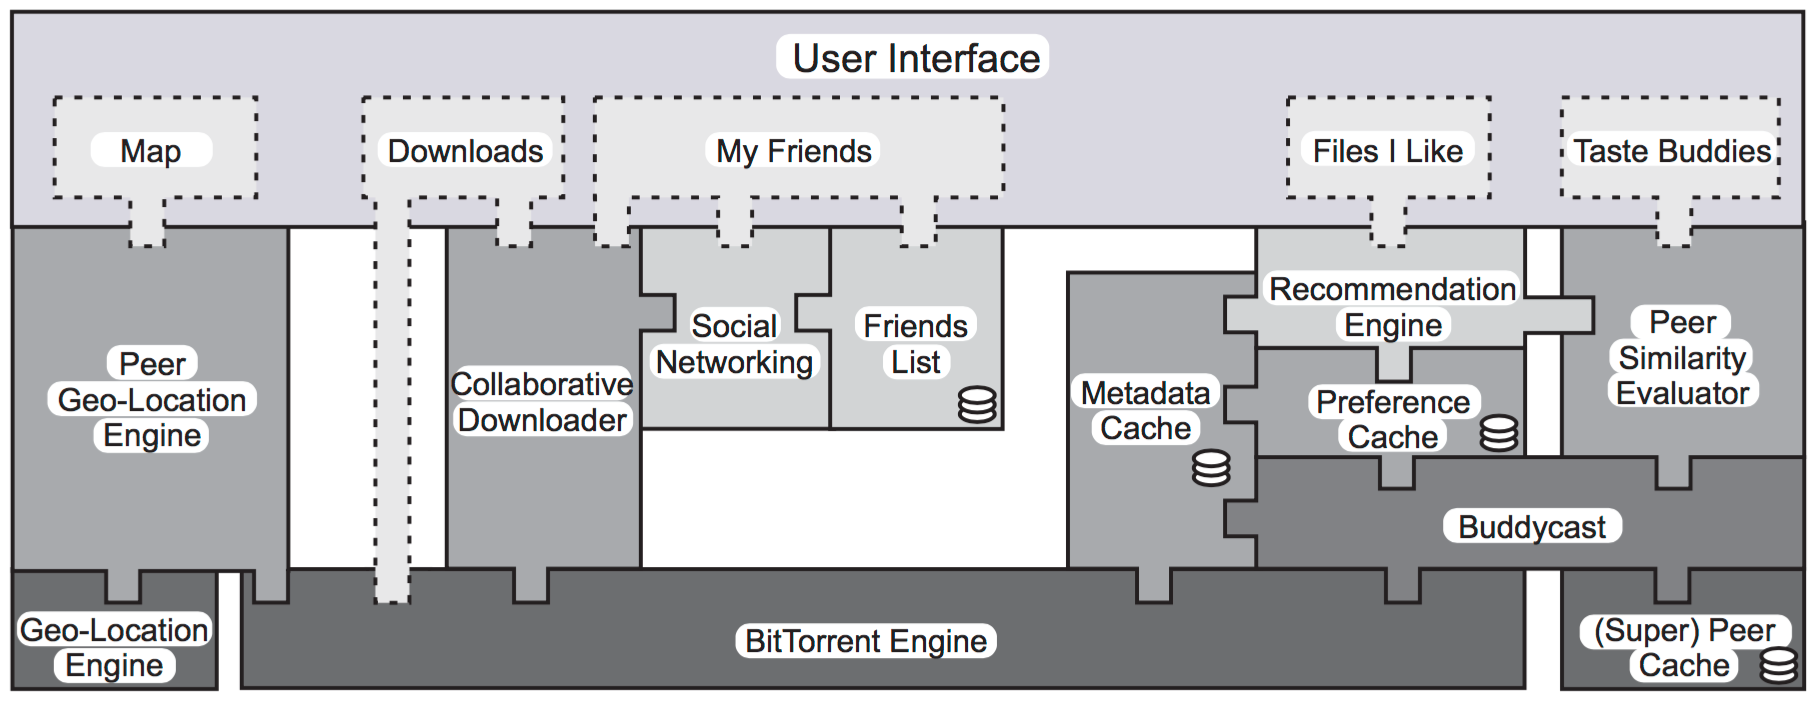
\includegraphics[width=1.0\columnwidth]{images/tribler_architecture_2007}
	\caption{The system architecture of Tribler as described in \cite{pouwelse2008tribler}.}
	\label{fig:tribler-architecture-2008}
\end{figure}

\subsection{Collaborative Downloads}
The BitTorrent engine provides tools to download and seed files in a decentralized way using a BitTorrent-compatible protocol. In addition, the module allows usage of the \emph{collaborative downloader} feature which significantly increases download speed by exploiting idle upload capacity of online friends in the network. The implemented protocol to facilitate these collaborative downloads is called \emph{2Fast} and it uses social groups where members who trust each other collaborate to improve their download performance.\\\\
The protocol works as follows: peers that are participating in a social group are either \emph{collectors} or \emph{helpers}. A collector is a peer that is interested in obtaining a complete copy of a particular file whereas a helper is a peer that is recruited by a collector to help downloading that file. Both types of peers start downloading a file using the regular BitTorrent protocol and the collaborative download extensions. However, before a helper tries to fetch a file piece in the network, it first asks the collector for approval which is granted when no other helpers have downloaded or are downloading the file piece in question already. Afterwards, the helper peer sends the piece to the collector. For ADSL and ADSL-2 internet connections, the maximum achievable speed-up is 4 and 8 times respectively.

\subsection{Geo-Location Engine}
In the left side of the architecture in Figure \ref{fig:tribler-architecture-2008}, we notice the \emph{Geo-Location Engine}, \emph{Peer Geo-Location Engine} and the map component in the user interface. The \emph{Geo-Location Engine} is used to determine the location of other peers in the torrent swarm, using an open  API\footnote{http://hostip.info}. The \emph{Peer Geo-Location Engine} has been built on top of this module, providing the primitives to display the location of peers on a map in the user interface. This feature stems from the goal to ease the process of visual identification of potential collaborators.

\subsection{Content Discovery and Recommendation}
The \emph{BuddyCast} algorithm is designed to serve recommendations to users and to enable peer and content discovery. BuddyCast is an epidemic protocol which works as follows: each peer in the network maintains a number of taste buddies with their content preference lists and a number of random peers, void of any information about their content preferences. Periodically, BuddyCast performs an \emph{exploration} or \emph{exploitation} step: when an exploration step is executed, the peer connects to one of its taste buddies. When an exploitation step is performed, the peer connects to a random peer in the network. When the connection with the other peer is successful, a \emph{BuddyCast} message is exchanged, containing the identities of a number of taste buddies along with their top-10 preference lists, a number of random peers, and the top-50 content preferences of the sending peer. The age of each peer is included in the message to help other users know about the "freshness" of peers. After the BuddyCast messages are exchanged, the received information is stored in the local database of each peer, called the \emph{Preference Cache}. Information about discovered peers are stored in the \emph{Peer Cache}. To limit the exchange of redundant information, each peer maintains a list of recently contacted peers.\\\\
The BuddyCast mechanism interacts with the user interface in two different ways. On the \emph{Files I Like} page in the interface, each peer indicates its preference for certain files expressed as a score between 1 and 5. Initially, this list is filled with the most recent downloads of the peers. Second, the user interfaces displays similar taste buddies and facilitates a content browser where each item is annotated with an estimated interest indicator for that user.

\section{Tribler between 2007 and 2012}
The first version of Tribler in the 4.x series, Tribler 4.0, is released in 2007\cite{tribler4tf}. Many features from the 3.x release cycles are untouched and some new functionality have been added, most notable in the user interface. With a new embedded video player, users can play videos (while being downloaded) directly from within the user interface. This video player is powered by the popular \emph{VLC} library\footnote{http://www.videolan.org/vlc/} and bindings that facilitates video management and playback in several popular user interface libraries. Tribler 4.0 allows users to remotely search for content inside the Tribler network but also searches content available on YouTube and Liveleak. These search results are presented to the user in a YouTube-like thumbnail grid. The user interface of Tribler 4.0 is displayed in Figure \ref{fig:tribler4}.\\

\begin{figure}[h!]
	\centering
	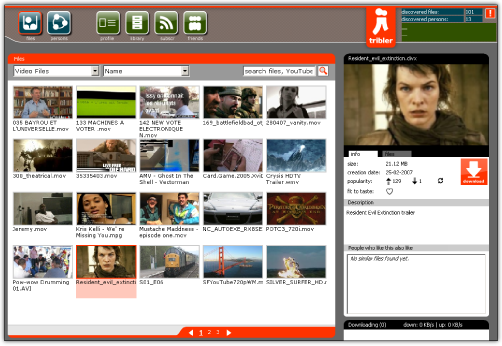
\includegraphics[width=1.0\columnwidth]{images/tribler4}
	\caption{The user interface of Tribler 4.0.}
	\label{fig:tribler4}
\end{figure}

The development of Tribler continued with the release of version 5.0 in 2009\cite{historyoftribler}. The user interface has been subject to a complete redesign, introducing a more dark theme, which was replaced by a white theme shortly after release. The focus of Tribler 5.0 has been on the stability and performance of remote content search and the download mechanism. The thumbnails have been dropped in favour of a paginated list.\\\\
Tribler 5.1 contained some major improvements to the user interface, thanks to the feedback of the community. A new, novel addition in Tribler 5.2 is the concepts of channels, similar to YouTube. One goal of the organization of content into channels was to prevent spam inside the network by favouring content present in more popular channels. Whereas custom widgets with an own look-and-feel has been used in this version, they all got replaced in Tribler 5.3 by native buttons to creating a more natural feel on each supported platform. Additionally, a tag cloud with popular keywords has been added to the home page of Tribler to help users determine which content they possibly want to look for. The paginated list was replaced by a single, scrollable list of items. In the next release, Tribler 5.4, a \emph{magic search} feature has been implemented where similar search results are collapsed using text similarity functions and digit extraction. The usefulness of this feature is apparent when searching for content that is split into many parts such as a sequel of books or a television show. This idea is that this feature leads to a much cleaner and comprehensive results list when searching for content.\\\\
The final release in the 5.x series, Tribler 5.9, bought some major additions. The complete BuddyCast core has been rewritten, moving away from a TCP overlay to an implementation based on UDP, providing benefits to the compatibility with \emph{Network Address Translation (NAT)} firewalls. Tribler adopted the \emph{Peer-to-peer streaming peer protocol (PPSPP)} protocol\cite{bakker2015peer}, implemented in \emph{libswift}, PPSPP provides download capabilities over UDP, thus removing the TCP layer from the BitTorrent engine.\\\\
The architecture around the time of Tribler version 5.5 is visible in Figure \ref{fig:tribler-core-architecture-55}. We notice that this architecture is significantly more complex compared to the design as presented in Figure \ref{fig:tribler-architecture-2008}. The depicted architecture excludes the user interface architecture which is equally complex. This model is the result of gradually adding and modifying smaller components to Tribler that have been developed during research, such as 2fast, BuddyCast and the \emph{Secure Overlay}, providing a high-level communication mechanism. We notice four different threads that need to work together, contributing to the complexity of the code since developers need to be aware of context switches (jumping between different threads during execution of the application). Whereas the project contained around 45.000 lines of code in 2007, this number has increased to over 90.000 in 2010.

\begin{figure}[h!]
	\centering
	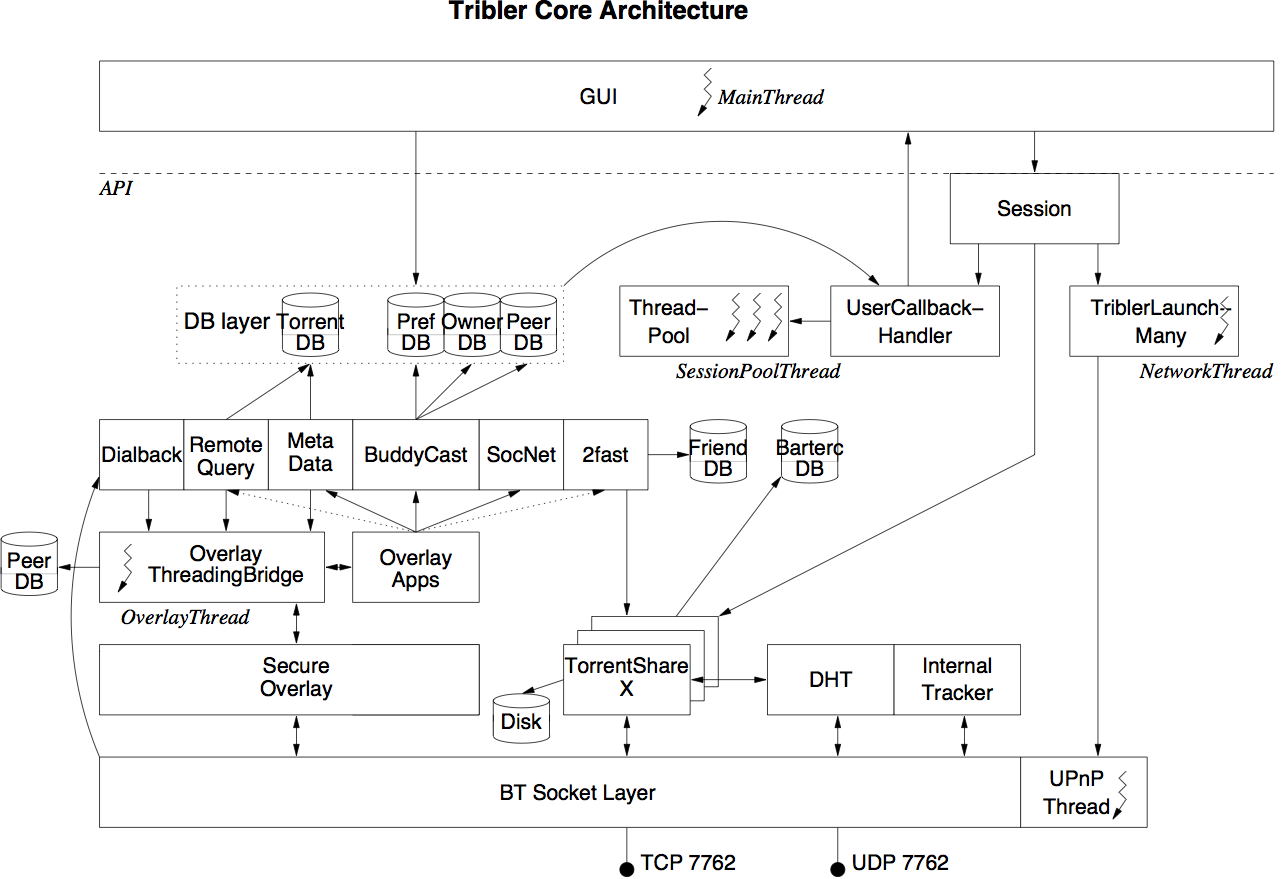
\includegraphics[width=1.0\columnwidth]{images/architecture/core_architecture_55}
	\caption{An overview of the core architecture around the time of Tribler 5.5.}
	\label{fig:tribler-core-architecture-55}
\end{figure}

\section{Tribler between 2012 and 2016}
Shortly after the release of Tribler 5.9, version 6.0 is released where a complete new user interface has been implemented and the PPSPP protocol implementation is replaced by the \emph{libtorrent} library, written in C++\footnote{https://github.com/arvidn/libtorrent}. This release also contained some minor bug fixes that increased performance and usability in general. After the release of version 6.0, several smaller releases (6.1, 6.2 and 6.3) followed. The focus of the Tribler platform shifted toward anonymous downloads and end-to-end encryption, designed and implemented by Plak, Tanaskoski and Ruigrok in 2014 and 2015\cite{plak2014anonymous}\cite{tanaskoski2014anonymous}\cite{ruigrok2015bittorrent}. The Tribler 6.4 release provided an experimental anonymous download mechanism and hidden seeding services implementation. Additionally, the release also introduced the \emph{Trivial File Transfer Protocol (TFTP)}, a simplistic version of the popular \emph{File Transfer Protocol (FTP)}. TFTP in Tribler is utilized to exchange torrent files between peers in Tribler when searching for content. The next release, Tribler 6.4.1, contained some major security fixes after an external code review by a member on the Tor mailing list\cite{githubissue1066}.

\subsection{Dispersy}
With the release of Tribler 6.1, \emph{Dispersy} got introduced. Described in \cite{zeilemaker2013dispersy} and mainly developed by Zeilemaker and Schoon, Dispersy lies at the foundations of the messaging and synchronization system in Tribler and is designed to deliver messages reliably in unpredictable networks. It provides a NAT traversal mechanism to improve the extent to which users are connectible in the network. Dispersy provides tools to quickly create distinct overlay networks, called \emph{communities}, that peers can join and where messages be exchanged. The communities as utilized by Tribler, together with a short description, is presented in Table \ref{table:dispersy-communities}. While being a major dependency of Tribler, a throughout analysis of Dispersy is considered outside the scope of this thesis.

\begin{table}
	\begin{tabularx}{\textwidth}{|l|X|}
		\hline
		\textbf{Community name} & \textbf{Purpose} \\ \hline
		\emph{AllChannel} & Used to discover new channels and to perform remote channel search operations.\\ \hline
		\emph{BarterCast4} & While currently disabled, this community was used to spread statistics about the upload and download rates of peers inside the network and created as mechanism to prevent free-riding in Tribler\cite{meulpolder2009bartercast}.\\ \hline
		\emph{Channel} & This community represents a single channel and is responsible for managing torrents and playlists inside that channel.\\ \hline
		\emph{Multichain} & The Multichain community utilizes blockchain technology and can be regarded as the accountant mechanism that keeps track of shared and used bandwidth.\\ \hline
		\emph{Search} & This community contains functionalities to perform remote keyword searches for torrents and torrent collecting operations.\\ \hline
		\emph{(Hidden)TunnelCommunity} & The (hidden) tunnel community contains the implementation of the Tor-like protocol that enables anonymity when downloading content and contains the foundations of the hidden seeder services protocol, used for anonymous seeding.\\ \hline
	\end{tabularx}
	\caption{An overview and description of implemented Dispersy communities in Tribler as of July 2016.}
	\label{table:dispersy-communities}
\end{table}

\subsection{Twisted}
\label{subsec:architecture-twisted}
In 2014, it was decided to make significant changes to the architecture by utilizing Twisted, an event-driven networking engine written in Python\footnote{https://twistedmatrix.com/trac/}. Twisted allows programmers to write code in an asynchronous way. The utilization of Twisted has been motivated by the presence of callback mechanisms in Tribler as can be identified in Figure \ref{fig:tribler-core-architecture-55}. The library provides a simple model for handling callbacks and events. At the heart of Twisted, we find the \emph{reactor} which is the implementation of the event loop\cite{twistedreactoroverview}. The event loop is a programming construct that waits for and dispatches events or messages in an application.
The threading model as available in Tribler 6 has been illustrated in Figure \ref{fig:old-threading-model}. In most applications that are using the Twisted library, the reactor operates on the main thread of a Python application. In Tribler, the reactor runs on a separate thread since the main thread is occupied by the event loop of \emph{wxPython}, the library used to built the user interface. This means that code performing operations with the user interface such as refresh operations of lists, should always be executed on the Python main thread. Operations that are using Twisted constructs however, should be scheduled on the reactor thread to function correctly. The Twisted threadpool provides a pool of additional threads to dispatch work to and can be utilized for longer-running operations that should not block the main or reactor thread. To make context switching more easy to implement, several method decorators have been implemented by Tribler developers, visible in Figure \ref{fig:old-threading-model}.\\\\
Developers should always be aware of the threading context when implementing new features. Long blocking calls on the main thread should be avoided as much as possible since they lead to an unresponsive user interface. Database calls however, should be scheduled on the reactor thread. While this architecture reduced the number of threads if we compare it to Figure \ref{fig:tribler-core-architecture-55}, we are still stuck with a dedicated thread for the reactor and complex thread switching patterns.

\begin{figure}[h!]
	\centering
	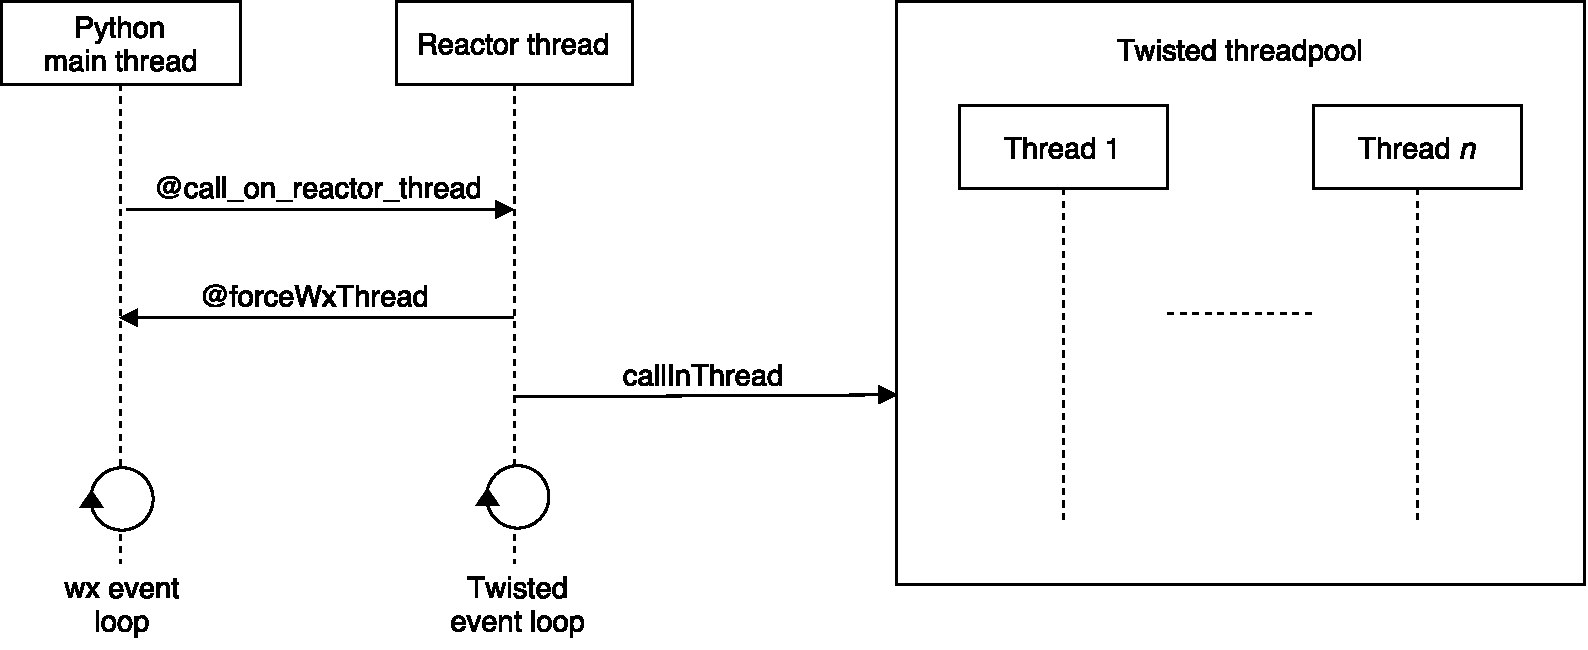
\includegraphics[width=1.0\columnwidth]{images/architecture/threading_model_tribler}
	\caption{The threading model used by Tribler 6, together with the primitives to schedule operations on different threads.}
	\label{fig:old-threading-model}
\end{figure}

\section{The roadmap of Tribler}
\label{sec:tribler-roadmap}
In the previous Section, the evolution of Tribler has been discussed. We have illustrated the increased complexity over time in terms of the architecture, design and threading model. We now turn our attention to the future of Tribler and propose a new architecture where we address some of the design flaws introduced in previous development iterations of Tribler. This new architecture should prepare Tribler for another ten year of research. We start by defining three requirements that our new architecture should meet:
\begin{itemize}
	\item \emph{simplicity}: we wish to shift towards an architecture that has a better learning curve for new developers. The current architecture is hard to learn, prone to errors and has a complex threading model, increasing the time for new developers to get familiar with the code. By modifying the architecture to make it simpler, we can save developer time and increase the chance for contributions from external developers outside the Tribler organization.\\\\
	Creating a simplified architecture inevitably leads to decisions to remove unnecessary, unused or broken components. The current architecture has various features for which we believe that the maintenance costs outweighs the benefits of that particular feature for end users. Making decisions to remove components and thus code, can lead to a significant reduction of technical debt.
	\item \emph{flexibility}: by introducing a substantial level of flexibility in the system, developers can focus on the development of individual components when contributing to Tribler. While we can identify many different modules in Figure \ref{fig:tribler-core-architecture-55}, there still are numerous interdependencies between them, making it hard to modify and test parts of the system in isolation. We propose a methodology based on component-based software engineering, where we provide interfaces between components to communicate with each other. The user interface should be implemented as a separate component, in comparison to the current architecture where the core and user interface cannot be used as separate modules (this will be elaborated in more detail in Chapter \ref{subsec:gui-core-packages}).
	\item \emph{performance}: Tribler contains various time-critical components that should work reliably and fast such as the download engine, the anonymous overlay and the content discovery mechanisms. Several development tasks have been conducted, focused on performance optimization of individual components or the system as whole.\\\\
	The new architecture should be designed with future performance engineering in mind. An unclear and unstructured architecture can cause much overhead for developers when boosting performance as is for instance illustrated by the numerous thread switching necessaries to implement a specific feature that utilizes both the Tribler core and user interface. By considering performance engineering as early in the process, we can build our architecture to allow for performance modifications.
\end{itemize}
We propose the architecture depicted in Figure \ref{fig:tribler7} which design follows a layered, component-based approach. The remainder of this Section will discuss the components in the architecture in more detail and highlight decisions that have been made during the design process.

\begin{figure}[h!]
	\centering
	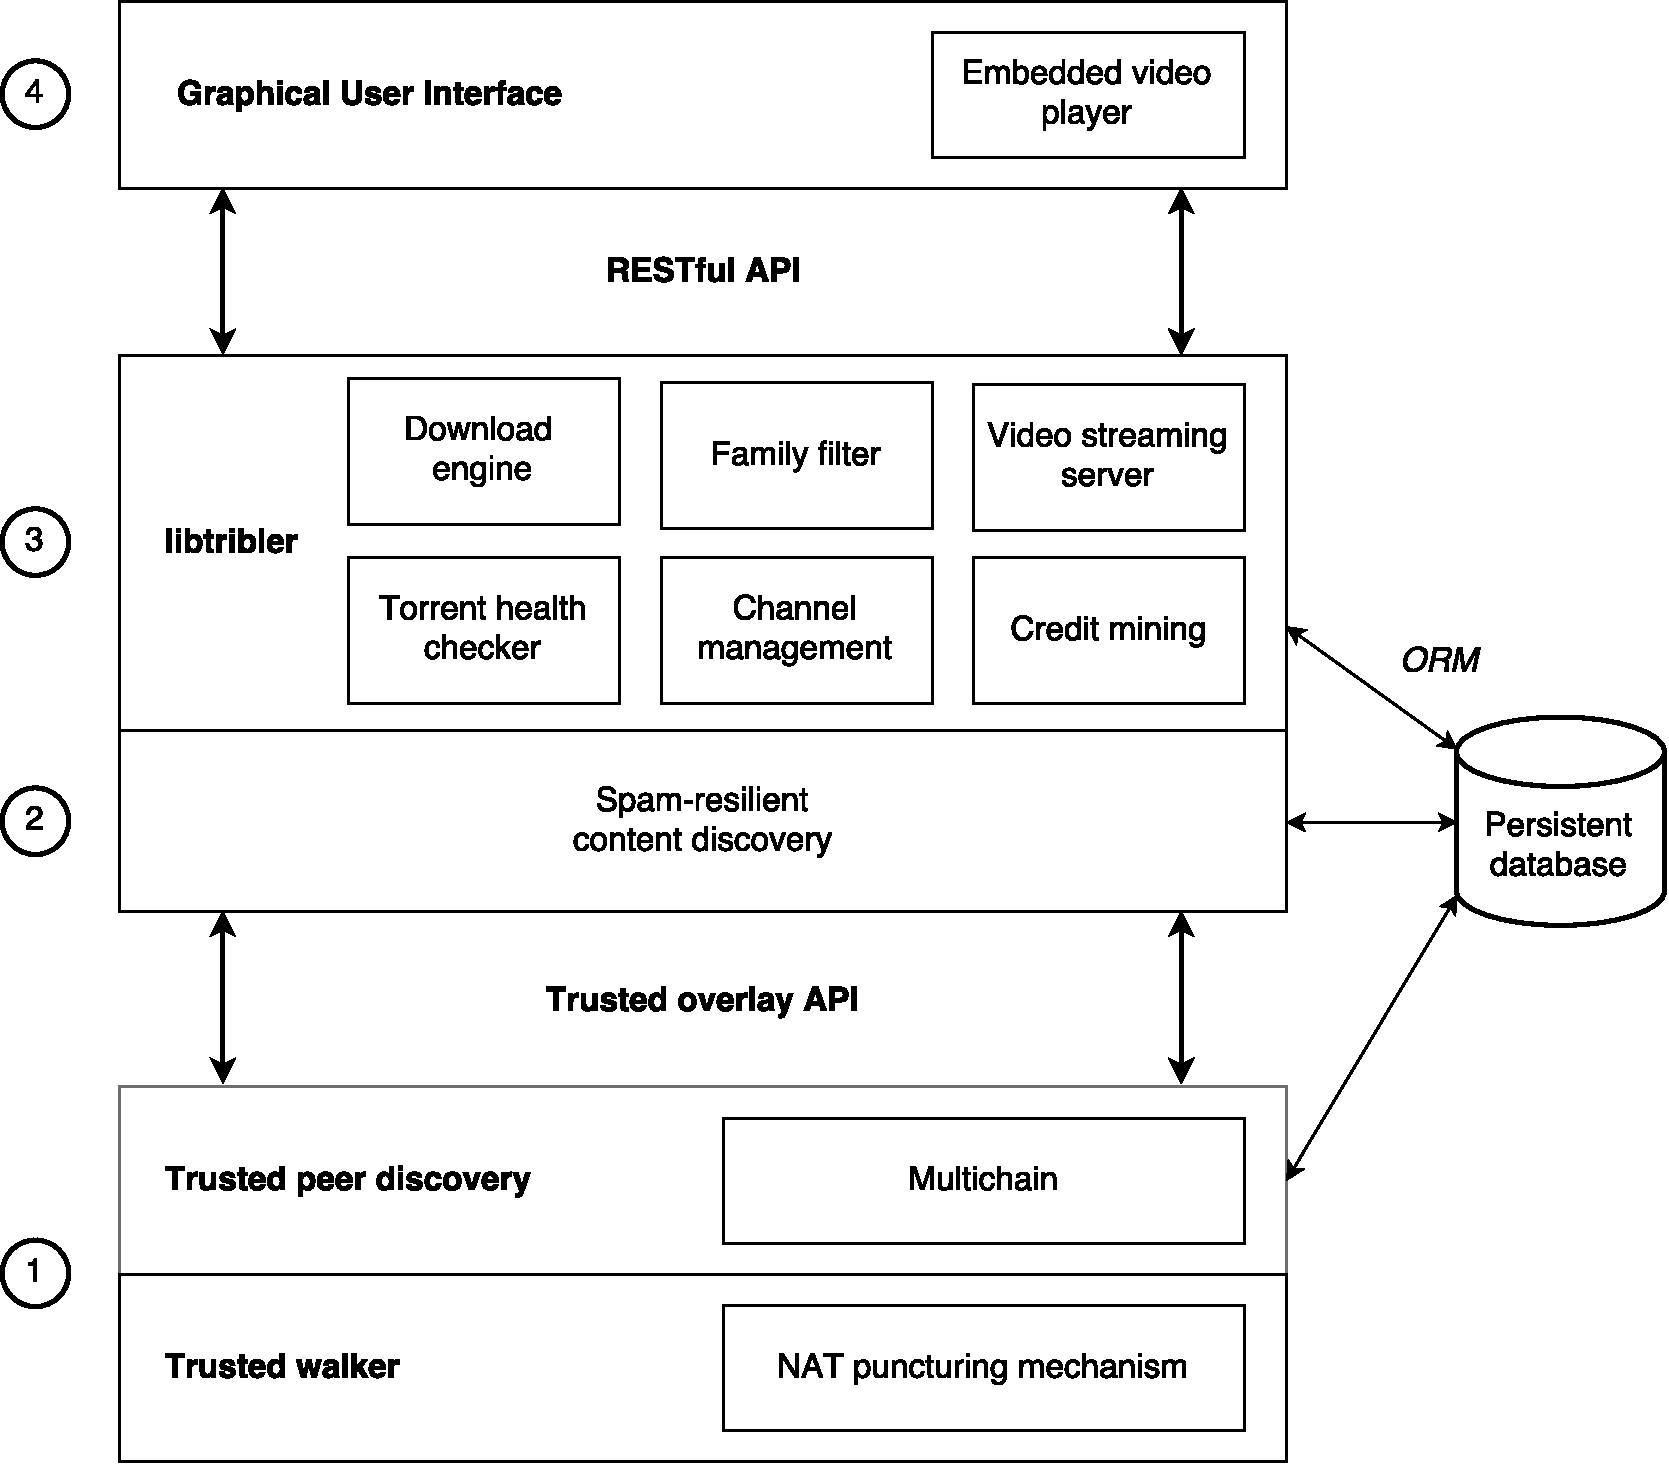
\includegraphics[width=0.9\columnwidth]{images/architecture/tribler7}
	\caption{The proposed architecture of Tribler 7, consisting of a trusted overlay (1), a content-discovery mechanism (2), \emph{libtribler} (3) and a user interface (4).}
	\label{fig:tribler7}
\end{figure}

\subsection{Trusted Overlay}
The trusted overlay is the lowest layer in Tribler that provides primitives for discovering and picking new trusted peers in the network. At the lowest level of the trusted overlay, we identify the trusted walker, the central component for discovering other peers. Currently, the Dispersy framework is responsible for discovering new peers within the Tribler network, using a gossiping protocol\cite{zeilemaker2013dispersy}. This discovery mechanism is illustrated in Figure \ref{fig:dispersy-discover} and executed at fixed time intervals. It works as follows: suppose node \emph{A} wants to discover an additional peer. First, he sends an \emph{introduction-request} to a random peer he knows, say node \emph{B}. Node \emph{B} now replies with an \emph{introduction-reply} message, containing information about a node that \emph{B} knows, in this case node \emph{C}. Meanwhile, node \emph{B} sends a \emph{puncture-request} message to node \emph{C} which in turn punctures the NAT firewall of node \emph{A}, making sure that node \emph{A} can connect to him. This algorithm both provides a NAT-puncturing mechanism and allows a node to discover new peers.\\

\begin{figure}[h!]
	\centering
	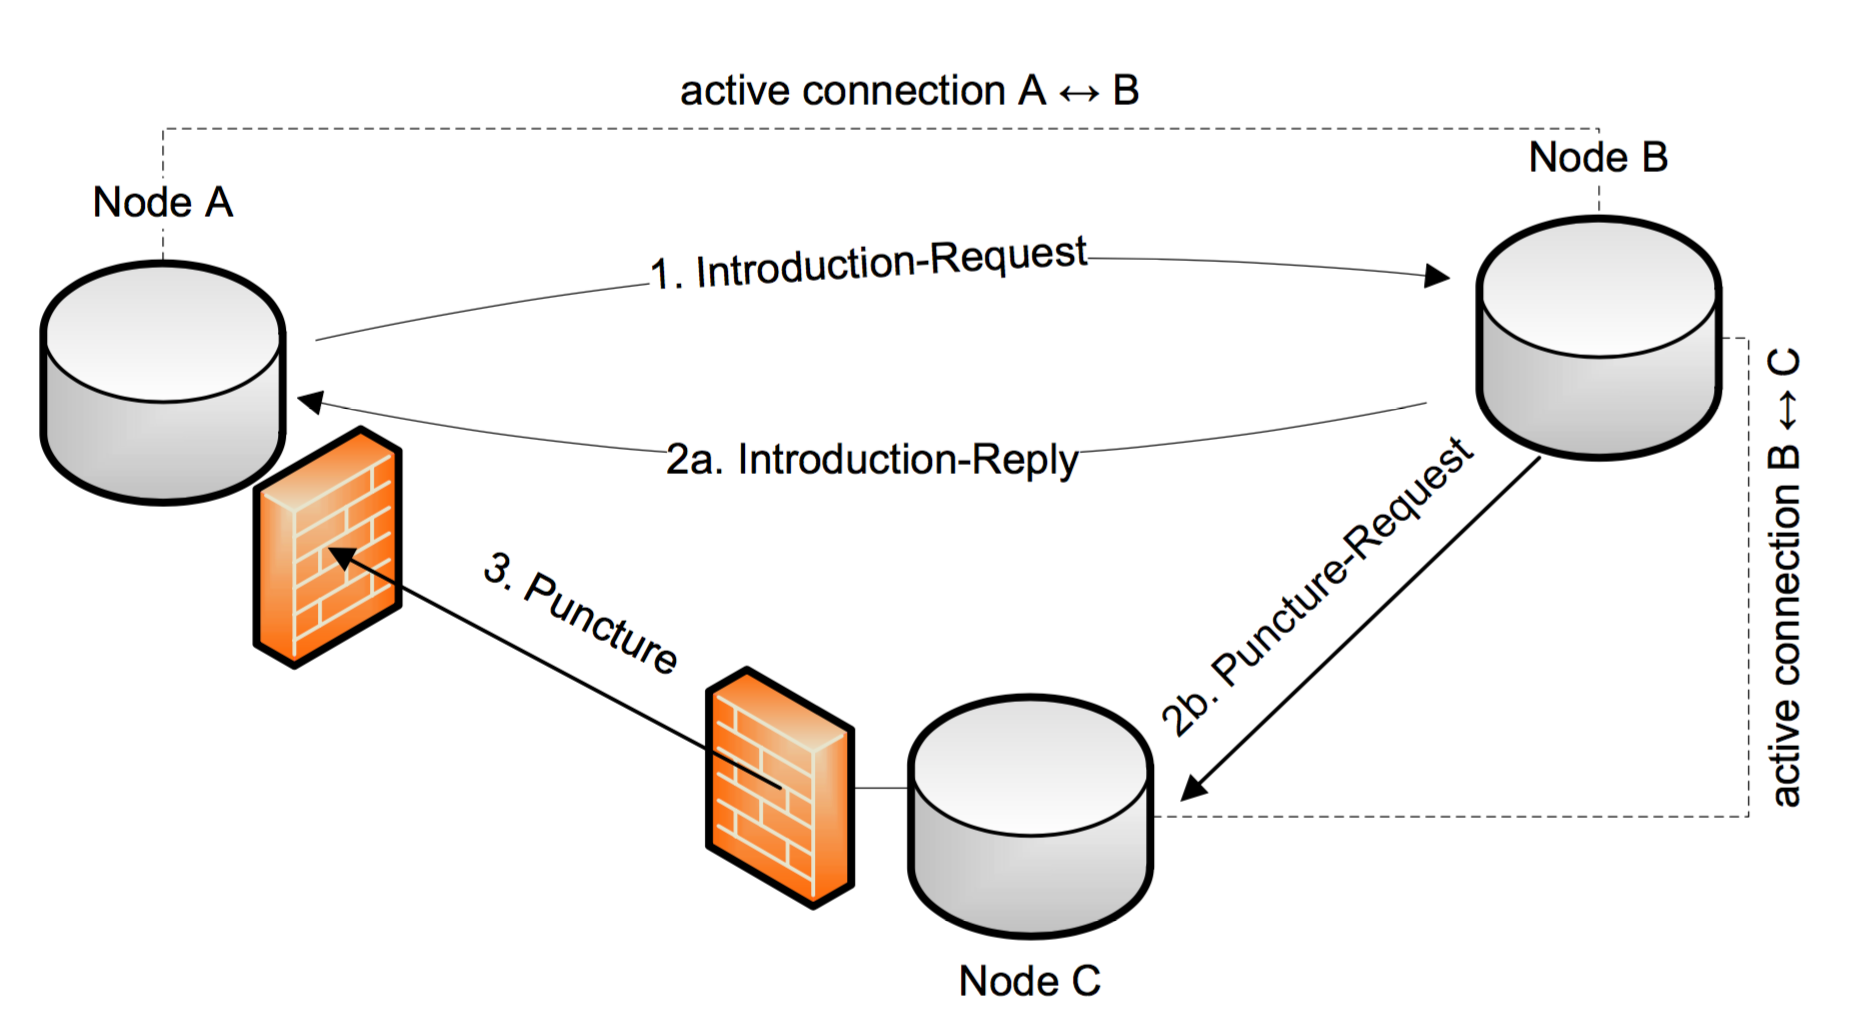
\includegraphics[width=0.7\columnwidth]{images/architecture/dispersy_discover}
	\caption{The discovery and NAT puncture mechanism as implemented in Dispersy.}
	\label{fig:dispersy-discover}
\end{figure}

The described mechanism of discovering new peers using Dispersy will be replaced by a trusted walker that uses accumulated reputation in the \emph{Multichain}, the accountant mechanism that keeps track of shared and used bandwidth, providing more reputation when a user provides upload capacity to help other users. The key idea is that \emph{sybil} nodes, forged identities in the network, and free riders are ignored and not considered as a trusted peer since their reputation is low and are not likely to be selected by the trusted walker.\\\\
New peers in that network that have not accumulated any reputation yet, start out by creating some random interactions with other nodes while learning about the network and the amount of reputation of other users. With an interval, every node runs an algorithm to calculate the reputation of their known peers. The amount of uploaded data does not have to be the only factor of this reputation mechanism: the uptime of the user in question can also be considered, where a higher uptime might lead to a better reputation and thus a higher trustworthiness. This leads to a trust network where each node knows about other trusted peers with which they can exchange content.\\\\
Interaction with the trust overlay can be realised by using an higher-level Application Programming Interface (API) which provides the facilities to perform operations regarding the discover of new trusted peers and management of known ones. By providing a trusted overlay API, the component allows for easy reuse which is beneficial when the module will be published as an open-source project.

\subsection{Spam-Resilient Content Discovery}
Discovering content is a key feature of Tribler. The spam-resilient content discovery component allows users to discover and search torrents, channels and playlists in Tribler using peers are managed by the trust overlay. The current implemented mechanism for information exchange in Tribler where messages are exchanged within segregated communities works well enough for this purpose, except for the exchange of more exotic  meta data such as content thumbnails. Providing users with a visual preview of content in the form of thumbnails is a good way to make the user interface more appealing, however, a robust implementation in a complete decentralized network is challenging due to the fact that the content can be present in a huge volume, thus increasing the total size of the thumbnails. We wish to keep the overhead introduced by thumbnail synchronization to a minimum and we must have a decent filtering algorithm to avoid inappropriate imagery from being shown unexpectedly in the user interface. These features will be considered future work and not be discussed in the remainder of this thesis.

\subsection{libtribler}
\emph{libtribler} provides the primitives to developers to make use of the above described components and contains the implementation of a RESTful API that is used to communicate with libtribler. We will now discuss the components which together account for this layer.

\subsubsection{\textbf{Download Engine}}
The download engine is one of the most crucial parts in Tribler: before facilitated by the BitTorrent and libswift libraries, we currently use the open source \emph{libtorrent} library to facilitate decentralized downloads. libtorrent is written in C++, however bindings for various other programming languages such as Python, Go and Java are available. \emph{libtorrent} uses an alert mechanism to notify the application that is using the library about events, such as download state transitions, peer discovery in the torrent swarm or completion of a meta info lookup in the \emph{Distributed Hash Table (DHT)}. There are no solid arguments for replacing the current download engine with another library that allows for decentralized and anonymous downloads. Moreover, the current way \emph{libtorrent} is used in Tribler requires minimal changes to adhere to the proposed design, except for some optional refactoring of the current code.\\\\
We should note that the method to fetch peers from the DHT in libtorrent is private and not accessible from Python code. Under normal circumstances, this method only invoked by libtorrent, however, we manually call this method when performing a DHT lookup on behalf of another peer in the hidden services protocol, described in more detail in \cite{ruigrok2015bittorrent}. To still make it possible to perform a lookup of peers in the DHT, we make use of a third-party library, named \emph{pymdht}, an implementation of the Mainline DHT protocol, written in Python. This dependency is undesirable since it introduces extra complexity and load of the system. Effort should be made to make this desired method accessible in libtorrent so Tribler can get rid of the dependency.

\subsubsection{\textbf{Streaming Engine}}
\label{subsubsec:video-server}
The video streaming component streams the video data to a video player outside \emph{libtribler} after or during a download. The implemented video server in the current architecture listens for and serves HTTP requests and is implemented using the \emph{SimpleHTTPServer} library\footnote{https://docs.python.org/2/library/simplehttpserver.html}, a built-in Python module that can be used to implement a HTTP web server. The functioning of the video server is based on HTTP range requests, allowing the web server to serve a subset of a file when the user navigates to a random time position in a video.\\\\
The inner workings of the video player is illustrated in Figure \ref{fig:video-server} and works as follows: when the user starts playing a video in an external video player, the player performs a HTTP range request to the video server implemented in Tribler. This range request contains information in the header about the requested range of the video file. When the video server receives the request, it first checks whether the requested range has been downloaded by the download engine already. If so, the server returns the requested data to the client. If the requested range is not available, the video server notifies \emph{libtorrent} that the bytes in the requested range should be prioritized for download, reducing the latency before the requested range is completely available. When all pieces are downloaded, libtorrent notifies the video server about this event and the video server completes the request by sending the data to the client.\\

\begin{figure}[h!]
	\centering
	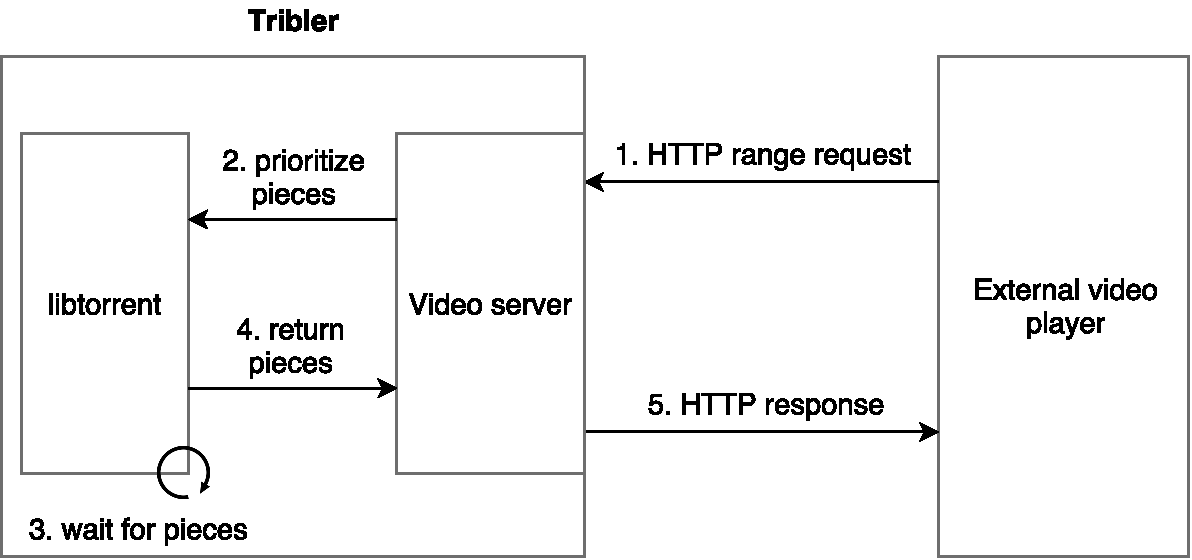
\includegraphics[width=0.7\columnwidth]{images/architecture/video_server}
	\caption{The flow when performing a HTTP range request when streaming a video using Tribler.}
	\label{fig:video-server}
\end{figure}

While the video server in the current form is functional, there is a performance improvement that can be considered: the video player runs on a separate thread and uses blocking calls to wait for the requested range to be downloaded. By integrating the video server inside the Twisted reactor thread, we can reduce the complexity of the server and utilize all of the facilities that Twisted provides, for instance, managing incoming requests. An additional consideration could be to run the video server in a dedicated process. This might increase the complexity since a communication mechanism between the Tribler and video server process is required to inform libtorrent about the prioritization of pieces.

\subsubsection{\textbf{Family filter}}
The freedom to upload any type of content in the network, comes with a price. The legal aspect of the available Tribler content can be disputable. While Tribler  contains legal content such as pornographic material, that content might be undesirable for most casual users. A mechanism called the family filter is  implemented in Tribler to filter out content that is not always safe for display. This filter is enabled by default and uses a list of keywords that can be associated with pornographic content. Discovered content gets classified by this filter, based on the torrent name, file names and other meta data. Unfortunately, this ad-hoc approach is not very effective since there are quite a few false positive classifications. While it provides some basic filtering tools, we noticed that the keyword-based approach can be greatly improved by using a more sophisticated classification approach. However, we would consider this as an enhancement rather than a defect that prevents a correct usage of Tribler.

\subsubsection{\textbf{Credit Mining}}
Ongoing work on a \emph{Credit Mining System (CMS)} in decentralized systems has been extensively described by the work of Capot\k{a} et al\cite{capotka2015decentralized} and is defined as the activity performed by peers for the purpose of earning credit. A possible purpose of the earned credits is to access exclusive content or receiving preferential download treatment in case of network congestion. Although the credit mining component is not enabled for end-users, a CMS has been implemented in Tribler, responsible for contributing bandwidth to the community without any intervention of the user. This mechanism is displayed in Figure \ref{fig:credit-mining} and works as follows: first, the user selects a source of swarms for the CMS to take in consideration. Possible sources are Tribler channels, RSS feeds or a directory containing one or more torrent files. Next, the CMS periodically selects a subset of the chosen swarms by the user. Finally, Tribler joins the swarms and tries to maximize earned credits by downloading as little as possible and maximizing the amount of uploaded data.\\

\begin{figure}[h!]
	\centering
	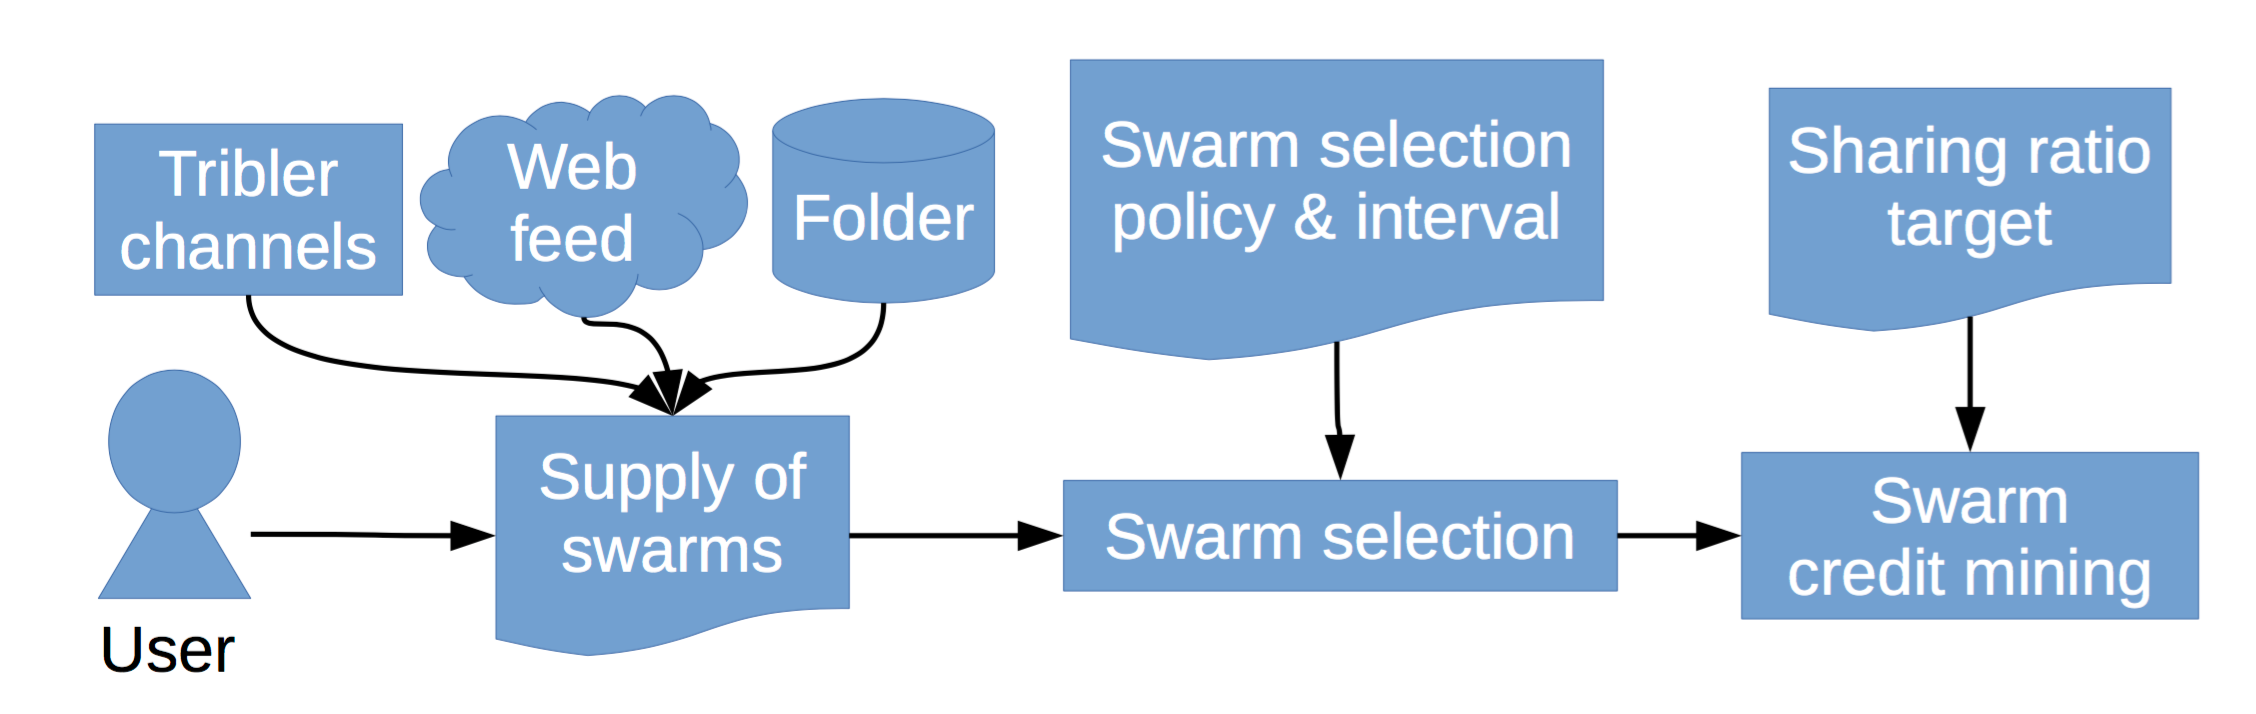
\includegraphics[width=0.7\columnwidth]{images/architecture/credit_mining}
	\caption{The credit mining system described in the work of Capot\k{a} et al.\cite{capotka2015decentralized}}
	\label{fig:credit-mining}
\end{figure}

The CMS can apply different policies for swarm selection. The first policy is to selects a swarm with the lowest ratio of seeders to all peers (leechers and seeders). Intuitively, this boosts swarms that are under-supplied (having a low amount of seeders). The second policy is to select swarms based on the swarm age. The intuition behind this policy is that newer content is often better seeded so it might be more beneficial to boost older swarms. The final policy that can be used is a random policy that selects a swarm using an uniform distribution.\\\\
This credit mechanism is a convenient way for users to increase their reputation by supplying bandwidth to the community, requiring minimal intervention of the user. The CMS works in conjunction with the Multichain which can be used as accounting tool to keep track of downloaded and uploaded bytes.

\subsubsection{\textbf{Channel Management}}
Tribler allows users to create their own channel and share content within that channel. Content can be shared in the form of torrents and playlists where a playlist is composed of a bundle of potential related torrent, for instance, some episodes of a tv show. Users can add content to the channels of other users, providing that the owner of the channel has set the status of the channel to \emph{open}.

\subsection{Communication between the GUI and libtribler}
\label{subsec:communication-gui-libtribler}
The communication between the upper level of the Tribler architecture, the GUI and libtribler should be facilitated by a \emph{Representational State Transfer (REST)} API. The REST architecture was introduced and defined by Roy Fielding in 2000\cite{fielding2000fielding} and is used frequently when building APIs that operate on the World Wide Web. A service that conforms to the REST architecture, is called RESTful.\\\\
In a RESTful architecture, resources and collections, identified by a Uniform Resource Identifiers (URIs) are returned by servers to clients. Common HTTP verbs (\emph{GET}, \emph{POST}, \emph{PUT} and \emph{DELETE}) are used to manipulate or retrieve these resources and collections. Table \ref{table:rest-api-operations} provides a summary of the most common operations that are used in a RESTful API.\\

\begin{table}[h!]
	\centering
	\begin{tabularx}{\textwidth}{|X|X|X|X|X|}
		\hline
		\textbf{Resource type} & \textbf{GET} & \textbf{PUT} & \textbf{POST} & \textbf{DELETE} \\ \hline
		\emph{Collection} & Retrieve the collection. & Replace the collection. & Create a new entry in the collection. & Delete the collection.\\ \hline
		\emph{Item} & Retrieve the item. & Replace the item, create it if it does not exist yet. & \emph{Often not used.} & Delete the item.\\ \hline
	\end{tabularx}
	\caption{A summary of REST verbs and their usage when dealing with a resource collection or a single item.}
	\label{table:rest-api-operations}
\end{table}

Prior to implementation of this API, we can already define some of the resources and collections. In Tribler, we can identify torrents, channels, playlists and downloads as collections that should be available for retrieval or modification using the API. Other than that, we might define a \emph{debug} collection that contains various statistics that are tracked by Tribler so developers can build debug tools which can be helpful during development or performance measurements.\\\\
A REST API provides a flexible and high-level interface that allows developers to write applications that are using Tribler, ranging from a command-line interface (CLI) to appealing user interfaces. Moreover, the implementation of these utility applications is not bound to a specific programming language, providing a huge amount of implementation freedom for developers. Moreover, it allows to run the these applications and Tribler in separate environments, improving responsiveness, performance and testability.

\subsection{Graphical User Interface}
At the highest level of the Tribler architecture stack, we find the user interface. The user interface should be able to communicate with the Tribler core using the RESTful API as described in the previous Subsection. A critical component of the user interface is the ability to play and control a video. The current user interface uses the \emph{wxPython} bindings to the VLC player, however, these bindings are not functional on MacOS due to platform incompatibilities.\\\\
The implementation of this interface is not limited to one programming language, however, to be able to reuse prior-existing code in the Tribler code base, it is a decent choice to write the interface in Python. Since the programming language is high-level and relatively easy to learn, new developers can easily make modifications to the user interface. We might also consider to refactor the current user interface to support the API. This consideration will be analysed in more detail in Chapter \ref{chapter:towards-new-architecture}. 

\subsection{Requirements Conformance}
In Section \ref{sec:tribler-roadmap}, we defined three requirements that our architecture should meet: simplicity, flexibility and a focus on performance. After the proposal and discussion of the new architecture, we will now evaluate to what extent our proposed design meets the requirements we composed.

\subsubsection{\textbf{Simplicity}}
Our first requirement was simplicity. The architecture as depicted in Figure \ref{fig:tribler-core-architecture-55} is complex and has a steep learning curve for new developers. The threading model as present in Tribler 6, requires developers to be sufficient aware about the thread on which specific operations should be scheduled, possibly leading to confusing code. The proposed architecture is simpler by design and more divided into separate components, increasing re-usability and testability. When modifying a specific component in a layer, developers should not have to care about the layers below the layer that is being modified. In this sense, the architecture meets our requirement that it should be more comprehensible and usable for developers.

\subsubsection{\textbf{Flexibility}}
The APIs that are facilitating communication between the layers in the architecture, increases the flexibility. As described in Subsection \ref{subsec:communication-gui-libtribler}, the RESTful API allows a great amount of flexibility for developers. We strive towards an implementation where individual components can easily be toggled using a configuration file by developers. Some components should also be configured by users, such as the credit mining mechanism.

\subsubsection{\textbf{Performance}}
One addition reason to split the architecture into different components, is based on performance engineering efforts performed on the system. By having components that are communicating with each other through an API, we are able to more easily extract and refactor these parts of the system in separate processes later on, thus increasing performance since different processes can utilize more CPU cores.